\subsection{Methods of Modelling Phages and Bacteria}
There are numerous ways to model the interactions between phages and bacteria. Models can be built at a molecular level, where the model simulates the mechanical and chemical behavior of a phage as it interacts with the surface of a bacterium using computational chemistry methods. On the other end of the spectrum, a different type of model can be built where populations of phages, bacteria and bacteria can be modeled using Ordinary Differential Equations (ODEs) or Delay Differential Equations (DDEs). DDEs are similar to ODEs, except where when ODEs are calculating the values of the equations at time $t$ using time $t-1$, DDEs can, but don't have to, use the value of the equation at time $t-\tau$, where $1 \leq \tau \leq t$. \newline 

Each type of system has its pros and cons. With the molecular level model, the model is more complex and needs significantly more startup time, simulation time, and is in general much more complex. However, more information can be gained from the simulations and can guide research in creating phages for a certain type of bacteria. The ODE method is simpler and easier to set up, however it can only capture large population dynamics. Certain assumptions have to be made, for example $\omega$ percent of the bacteria population is washed out. The model can be made more complicated, by modelling each stage of a lysis, or when calculating the washout rate of bacteria, use a normally distributed variable $\textbf{N}(\mu=\omega, \sigma=1)$ to capture slight variations in a parameter at each step to controllably randomize parameter values to capture noise in measuring data. Ensuring the use of a seed value will ensure that each run of the model results in the same output. 

\subsubsection{Generalized Lotka-Voltera Model}
The Lotka-Voltera model, a first-order non-linear differential model is a model that captures the dynamics between predators and prey, with phages being the predator and bacteria being the prey. Any population can be modelled as such
\[ 
    \frac{d{B}_i}{dt} = {B}_i \left(\left(r_i + \sum_{j}^{N} \alpha_{ij}{B}_j \right) - m_i\right)
\]
where ... 

\subsubsection{Generalized Consumer-Resource Model}
The generalized Consumer-Resource Model models the growth of a population and resource dynamics between a population of bacteria ${B}_i$ and a resource ${R}_i$. 
\begin{align}
    \frac{d{B}_i}{dt} &= r_i{B}_i \left(\sum_{\alpha} \Delta w_{i \alpha}C_{i \alpha}R_{\alpha}\right) - m_i {B}_i \\
    \frac{R_{\beta}}{dt} &= -\sum_i C_{i\beta}R_{\beta}{B_i} + \sum_{\alpha, i}D_{\beta\alpha}^{i}C_{i\alpha}R_{\beta}{B}_i \\
    \Delta w_{i\alpha} &= \sum_{\beta}D_{\beta \alpha}^{i}w_{\beta}
\end{align}

\subsubsection{Trait-Based Model}
The Trait-Based Model is a model that takes into account external factors such as the temperature or pH of the system, and can be modeled as following:  
\begin{align}
    \frac{dB_i}{dt} &= \left(r_i - m_i\right) B_i \\
    r_i &= \frac{r_{i\alpha}^{max}R_\alpha}{R_\alpha + K_{i\alpha}}e^{S_i\left(T-T_{ref}\right)}
\end{align}
where $S_i$ is the sensitivity to $B_i$ to factor $T$, and with tradeoff if $r_i^{max} > \text{ mean } r^{max} \text{ then } S_i > \text{ mean } S$. 

\subsubsection{Agent-Based Models}
Agent-based Models (ABM) model the system through space and time. An $x \times y \times z$ grid (often $z$ is left out for a 2D system) is created and split into smaller subcells containing resources and microbes. Each cell acts as its own tiny environment, where resources and microbes interact within the environment, but not with the neighboring cells. Resources are diffused through the system using a PDE solver for a Boundary Value Problem (BVP). Agents are allowed to move into neighboring grids with a probability $p$, where $p$ can depend on any number of parameters such as nutrient density, microbe density, or stochastic chance. \newline 
ABMs are useful when simulating many individual elements interacting in a system. Chaotic or emergent behaviour can arise from these interactions. Chaotic behavior refers to the irregular and unpredictable evolution of a system's behavior due to nonlinear equations, exhibiting sensitive dependence on initial conditions \cite{encyclopedia_of_physical_science_and_technology}. \newline 
Emergent behavior is something that is a nonobvious side effect of bringing together a new combination of capabilities—whether related to goods or services. Emergent behaviors can be either beneficial, benign, or potentially harmful, but in all cases they are very difficult to foresee until they manifest themselves. Agents can have simple rules, but when interacting with other agents, behavior that hasn't been programmed can arise. Emergent behaviors are also sometimes considered to be systems that are more complex than the sum of their parts \cite{macaulayThreatsImpactsIoT2017}. 



\begin{align} 
    \frac{\delta R_\alpha(r, t)}{\delta t} = \nabla \left[D \left( R_\alpha, r\right) \nabla R_\alpha \left( r, t \right) \right], r = \left(x, y\right)
\end{align}. 
The cellular agents rules are as follows. 
\begin{align} 
    \frac{di}{dt} = r_i \left( \sum_\alpha \Delta w_{i\alpha}C_{i\alpha}R_\alpha\right)
\end{align}, where if $i>$ threshold, $\frac{i}{2}$ expands into the neighboring grid cell with a probability $p$. 
The resource consumption and conversion into new sub-resource types are described as follows. 
\begin{align}    
    \frac{dR_\alpha}{dt} &= -\sum_i C_{i\alpha}R_\alpha I \\
    \frac{dR_\beta}{dt} &= \sum_i C_{i\beta}R_\beta I + \sum_{\alpha, i}D_{\beta \alpha}^{i} C_{i \alpha} R_\alpha i
\end{align}






\subsection{Biology of Phages}
\subsubsection{Current Applications: Food Control}

When there are small number of known bacterial strains, a targeted concoction of phages can be used to control the bacterial population growth on the food. Phages offer properties of microbial control that other methods do not. Phages do not modify the food quality and do not leave behind harmful chemical residues. Phages are hyperspecific to the bacteria that they can kill, and they don't affect other beneficial bacteria. For example, \textit{Streptococcus thermophilus} is one of three different bacteria strains used to create emmental cheese. However, Emmental cheese does not use pasteurized milk, increasing the risk of \textit{E. coli}. Emmental cheese producers can add phages that target \textit{E. coli} to the milk during the production stage while not affecting the bacteria used to produce the cheese. \newline 


Phage cocktails like SalmoFresh\textsuperscript{TM} have been proven to safely reduce \textit{Salmonella} contamination in pet food and raw pet food ingredients \cite{sofferBacteriophagesSafelyReduce2016}, as well as in romaine lettuce and bean sprouts \cite{zhangSalmoFreshEffectivenessControlling2019}. Pet food contains meat and vegetables, where vegetables grown in or on the ground are at risk of \textit{Salmonella} due to contact with soil, manure, compost, and other agricultural runoff from neighboring farms \cite{kowalskaFreshVegetablesFruit2023}. \Cref{fig:SalmoFresh_pet_food} \cite{sofferBacteriophagesSafelyReduce2016} and \Cref{fig:SalmoFresh_lettuce} \cite{zhangSalmoFreshEffectivenessControlling2019} show how applications of phages have reduced the count of \textit{Salmonella} in ingredients used in pet food as well as romaine lettuce and bean sprouts. As such, phages can be shown to control the spread of \textit{Salmonella} in food sources. 

\begin{figure}
    \centering
    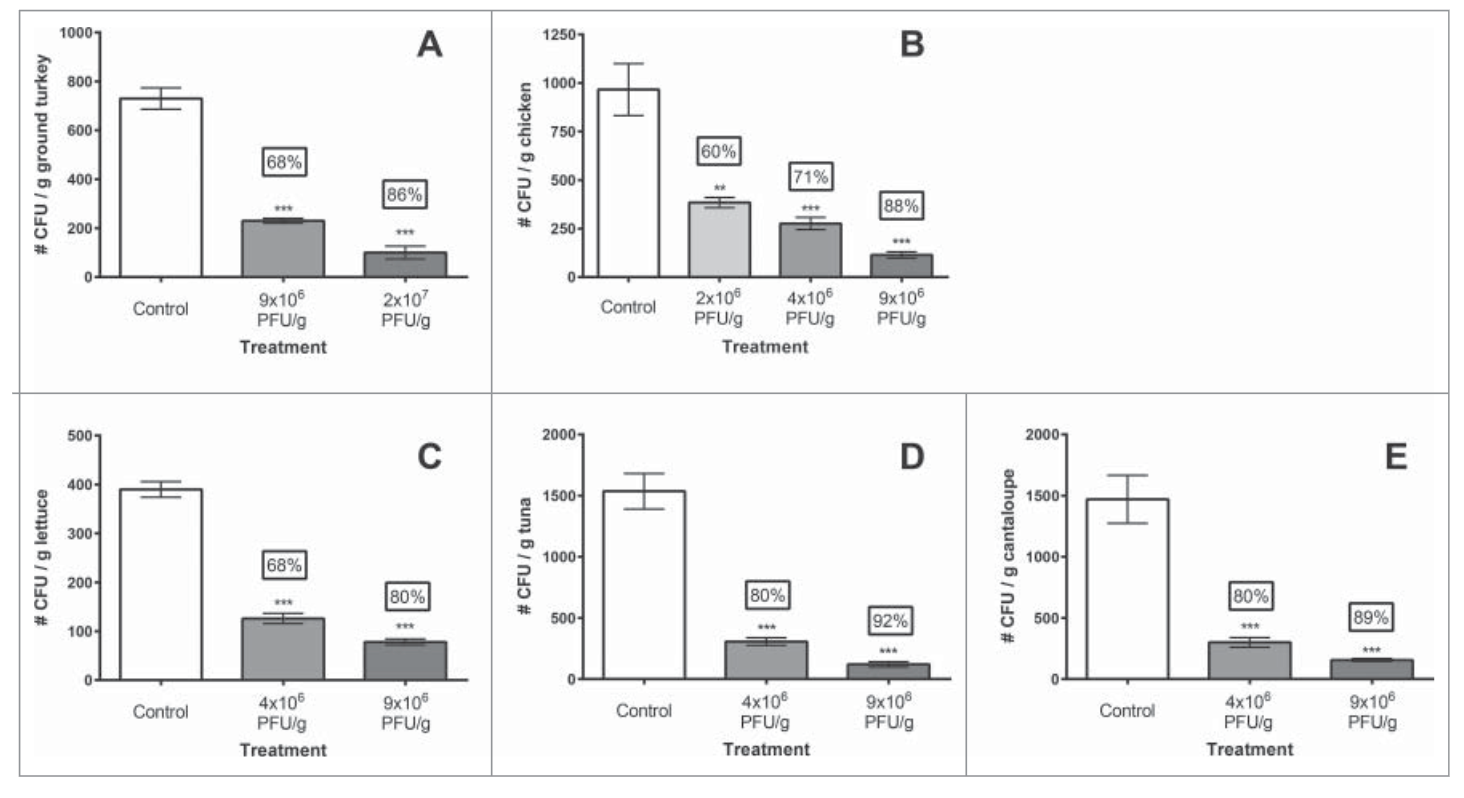
\includegraphics[width=0.5\linewidth]{Figures/SalmoFresh_in_pet_food.png}
    \caption{SalmoLyse\textsuperscript{\textregistered} reduces Salmonella contamination on various food surfaces: Mean and standard error bars shown. Statistical analyses were carried out for each food group independently. Asterisks denote significant reduction from corresponding controls based on one-way ANOVA with Tukey’s post-hoc tests for multiple corrections: ** denotes $p < 0.01$, while *** denotes $p < 0.001$ compared to the corresponding controls. There was significant reduction in Salmonella on all food surfaces with the addition of SalmoLyse\textsuperscript{\textregistered} compared to the controls; the mean percent reductions from the control are noted in the boxes above treatment bars. CFU/g D colony forming units per gram. Each letter denotes a food group that was tested with SalmoLyse\textsuperscript{\textregistered} and compared to a control: A= chicken; B= lettuce; C= tuna; D= cantaloupe; E= ground turkey. \cite{sofferBacteriophagesSafelyReduce2016}}
    \label{fig:SalmoFresh_pet_food}
\end{figure}

\begin{figure}
    \centering
    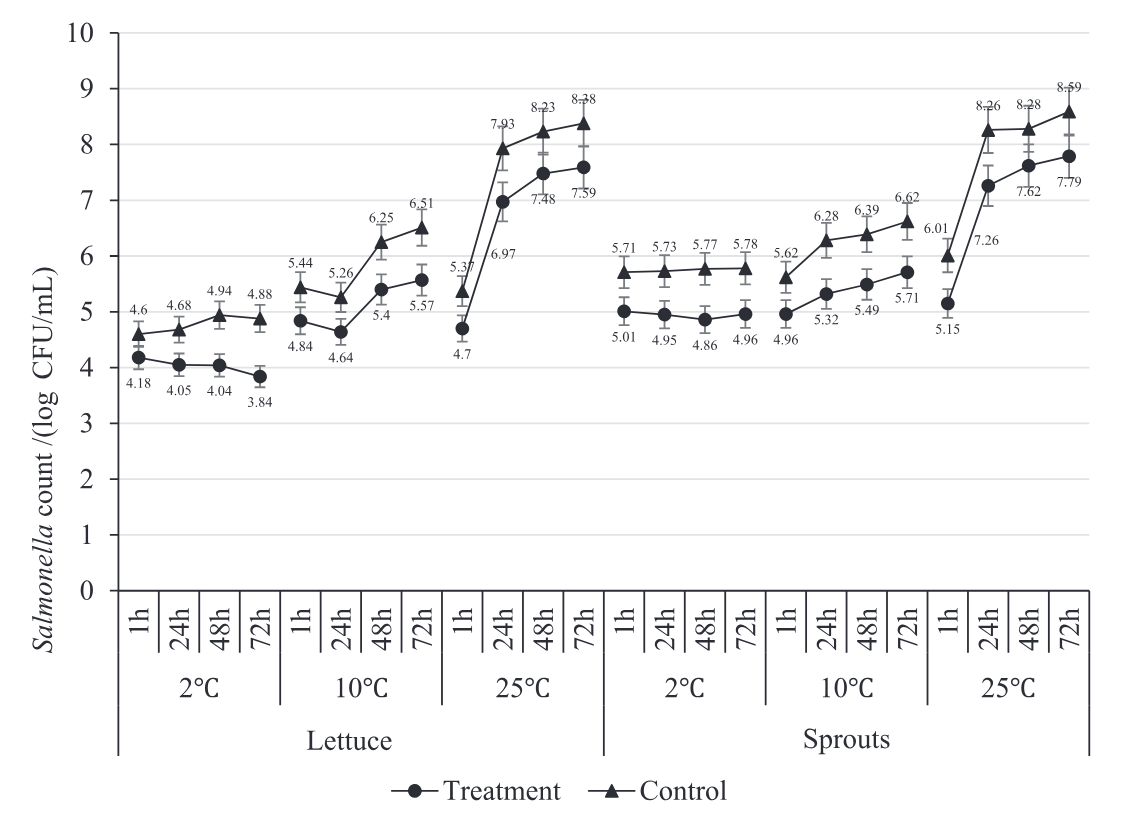
\includegraphics[width=0.5\linewidth]{Figures/SalmoFresh_effectiveness_lettuce_sprouts.png}
    \caption{\textit{Salmonella} count in a mixture of 5 \textit{Salmonella} strains spot-inoculated (CFU/g) onto a) lettuce and b) sprouts after spraying with a mixture of bacteriophage (SalmoFresh\textsuperscript{TM}) relative to positive controls at 2, 10 and 25C and stored for 1, 24, 48 and 72 h. \cite{zhangSalmoFreshEffectivenessControlling2019}}
    \label{fig:SalmoFresh_lettuce}
\end{figure}


\subsubsection{Current Applications: Bacterial Infection Control}


\subsubsection{Current Applications: Environmental Control}
There is interest in using phages to control cyanobacteria blooms. Phages can offer better and safer options than chemical options. Chemical options are indiscriminate, killing cyanobacteria, while also killing other beneficial bacteria and aquatic life. Although not used to control bacteria blooms, some chemicals like PFAS, also called "Forever Chemicals", can last a long time in the environment and don't degrade and keep on negatively affecting the environment. Due to the specificity of phages, only the cyanobacteria will be targeted, and will not affect the surrounding areas. Tucker and Pollard found that an isolated phage cocktail collected from Lake Baroon in Australia could decrease the abundance of \textit{M. aeruginosa} by 95\% within 6 days in a lab setting, before recovering within 3 weeks time \cite{tuckerIdentificationCyanophageMaLBP2005}. \newline 
There is evidence that phage-resistant bacteria can influence the population dynamics of other bacteria. It has been shown that the plankton level has been experimentally affected by the frequency of the phage-resistant \textit{Nodularia} marine bacteria. Populations with high phage resistance ($>50\%$) dominate the plankton communities despite a high phage count and eventually outcompete other bacteria due to their slower loss in population count. Contrastingly, populations of bacteria with low phage resistance (between 0\% and 5\%) were lysed to extinction, releasing nutrients like nitrogen. This allows for other bacterial strains to absorb the nutrients and dominate the bacterial community. Phages and the lysis of bacterial strains can have a dramatic effect on community dynamics and composition of other agents like phages, bacteria, and resources \cite{colomaFrequencyVirusresistantHosts2019}. Phages have the potential to be used as a highly specific strategy for the control of cyanobacterial blooms, with minimal effects to the environment, and offer control bacterial blooms, with limited impact to the environment. Usage should be relatively safe, novel, efficient, and sensitive. \newline 

However, there are issues with using phages to control bacterial blooms. Bacterial blooms can cover vast areas, or be in areas that would be hard to reach like marshlands, applying phages to combat the bloom might be infeasible. If the method of choice was to spray a solution of water containing phages, the solution needs to be shipped to the site and loaded onto special boats to  spray the solution into the water, or the trucks need to drive along the shore and spray the solution into the water. The phage density in the solution will have to be relatively high to quickly combat the bloom. These problems provide major logistical problems with creating the phages in a lab or factory, transporting the phages, and finally the administration of the phages to the waterways. Phages can only diffuse through the water, and can't actively swim, so they are dependent on the rate of diffusion and water currents. This will be difficult in marshlands, where the bacteria can "hide" in the grass and crevices created by aquatic life. If the bloom is in a high current area, like in a river or a bay, the water can wash the phages away. On top of that, The infection mechanism of phages is not exactly known, and research into artificial engineering of phages is not in-depth, making it harder to do research in this area \cite{grassoReviewCyanophageHost2022, DissolvedMicrocystinRelease}. 